\documentclass[a4paper,12pt]{article}
\usepackage{lmodern}

% --- Pacotes principais --- %
\usepackage[brazil]{babel}
\usepackage[utf8]{inputenc}
\usepackage[T1]{fontenc}
\usepackage{amsmath, amssymb}
\usepackage{enumitem}
% --- Fonte e layout otimizados para anotações ---
\usepackage[sfdefault]{sourcesanspro} % Fonte limpa e moderna
\usepackage[a4paper, left=2.3cm, right=2.3cm, top=2.8cm, bottom=2.8cm]{geometry}
\linespread{1.15} % ótimo espaçamento para leitura
\usepackage{xcolor}
\usepackage[most]{tcolorbox}
\usepackage{setspace}
\usepackage{tikz}
\usepackage{float}
\usepackage{colortbl}
\usepackage{array}
\usepackage{hyperref}
\usepackage{tocloft}
\usepackage[normalem]{ulem}
\usepackage{placeins}
\usepackage{fancyhdr}
\setlength{\headheight}{25pt}
\addtolength{\topmargin}{-10pt}

% --- Configuração de colunas ---
\newcolumntype{P}[1]{>{\centering\arraybackslash}p{#1}}

% --- Bibliotecas TikZ ---
\usetikzlibrary{trees, positioning}

% --- Estilo geral ---
\setstretch{1.15}
\setlength{\parskip}{0.5em}
\setlength{\parindent}{0pt}

% --- Espaçamento entre seções ---
\usepackage{titlesec}
\titlespacing*{\section}{0pt}{0.8em}{0.5em}
\titlespacing*{\subsection}{0pt}{0.6em}{0.3em}

% --- Configuração do sumário ---
\setlength{\cftbeforesecskip}{0.1em}
\setlength{\cftbeforesubsecskip}{0.05em}
\setlength{\cftbeforesubsubsecskip}{0.1em}

% --- Paleta preto e cinza ---
\definecolor{cinzaEscuro}{RGB}{40, 40, 40}
\definecolor{cinzaClaro}{RGB}{230, 230, 230}
\definecolor{cinzaMedio}{RGB}{120, 120, 120}
\definecolor{pretoFosco}{RGB}{15, 15, 15}

% --- Cores e estilo das seções ---
\usepackage{sectsty}
\sectionfont{\color{cinzaEscuro}\large\sffamily}
\subsectionfont{\color{cinzaMedio}\sffamily}
\subsubsectionfont{\color{cinzaMedio}\sffamily}

% --- Cabeçalho e rodapé ---
\pagestyle{fancy}
\fancyhf{}
\lhead{\textcolor{cinzaMedio}{\textbf{Introdução à Inteligência Artificial}}}
\rfoot{\textcolor{cinzaMedio}{\thepage}}
\renewcommand{\headrulewidth}{0.4pt}
\renewcommand{\footrulewidth}{0.4pt}
\renewcommand{\headrule}{\hbox to\headwidth{\color{cinzaClaro}\leaders\hrule height \headrulewidth\hfill}}
\renewcommand{\footrule}{\hbox to\headwidth{\color{cinzaClaro}\leaders\hrule height \footrulewidth\hfill}}

\fancypagestyle{plain}{%
  \fancyhf{}
  \lhead{\textcolor{cinzaMedio}{\textbf{Introdução à Inteligência Artificial}}}
  \rfoot{\textcolor{cinzaMedio}{\thepage}}
  \renewcommand{\headrulewidth}{0.4pt}
  \renewcommand{\footrulewidth}{0.4pt}
  \renewcommand{\headrule}{\hbox to\headwidth{\color{cinzaClaro}\leaders\hrule height \headrulewidth\hfill}}
  \renewcommand{\footrule}{\hbox to\headwidth{\color{cinzaClaro}\leaders\hrule height \footrulewidth\hfill}}
}


\begin{document}

% --- Título estilizado ---
% --- Título simples e elegante ---
\begin{center}
    \centering
    \vspace*{\fill}
    {\sffamily\bfseries\fontsize{28}{32}\selectfont\textcolor{pretoFosco}{Lógica Computacional}}\\[0.6em]
    \vspace*{\fill}
\end{center}

\pagestyle{fancy} 
\newpage

% --- Sumário --- %
\tableofcontents
\newpage

% --- Seções ---
\section{Introdução}

    \subsection{O que é a Internet?}

    Bilhões de dispositivos se conectam à Internet atualmente.

    \begin{itemize}
        \item \textbf{Hosts (sistemas finais) :} \\  
            $\hookrightarrow$ \underline{Exemplos:} smartphones, notebooks, máquinas servidoras, etc. \\  
            $\hookrightarrow$ Executam \textbf{aplicações de rede} e \textbf{interagem com o usuário}. 
        
        \item \textbf{Packet switches (comutadores de pacotes) :} \\          
            $\hookrightarrow$ Incluem \textbf{roteadores} e \textbf{switches}. \\  
            $\hookrightarrow$ Responsáveis por \underline{transportar pedaços de dados (pacotes)} de um ponto ao outro.

        \item \textbf{Communication links (enlaces de comunicação) :} \\  
            $\hookrightarrow$ Recursos necessários para conectar dispositivos (finais, switches, roteadores, etc.). \\  
            $\hookrightarrow$ Tipos: 
            \begin{itemize}
                \item \textbf{Cabeados:} fibra óptica, cobre.  
                \item \textbf{Sem fio:} Wi-Fi, satélite.
            \end{itemize}
            $\hookrightarrow$ \textbf{Taxa de transmissão:} também chamada de \underline{Banda}.

        \item \textbf{Redes :} \\  
            $\hookrightarrow$ Coleção de dispositivos e roteadores sob uma \underline{gerência centralizada} por uma instituição. \\  
            $\hookrightarrow$ \textbf{Tipos:}
            \begin{itemize}
                \item \textbf{Públicas:} padrões abertos, como HTTP, Ethernet.  
                \item \textbf{Proprietárias:} mantidas por instituições privadas, como o Skype.
            \end{itemize}

        \item \textbf{IETF (Internet Engineering Task Force) :}  \\
            $\hookrightarrow$ Responsável por \underline{gerenciar e controlar os padrões da Internet}. \\  
            $\hookrightarrow$ Cada padrão é lançado como um \textbf{RFC (Request for Comments)}. \\ 
            $\hookrightarrow$ Define e especifica as \textbf{características de um protocolo}. 
        
        \item \textbf{Internet como infraestrutura de serviços:}  \\
            $\hookrightarrow$ Provê serviços para \textbf{aplicações que executam em sistemas finais}. \\  
            $\hookrightarrow$ \underline{Exemplos:} web, streaming de vídeo, e-mail, jogos, redes sociais, etc. 
        
        \item \textbf{Interface de programação para aplicações distribuídas :} \\ 
            $\hookrightarrow$ Permite que uma aplicação \underline{envie mensagens pela Internet}. \\  
            $\hookrightarrow$ Garante que o receptor consiga \underline{receber a mensagem de forma apropriada}.

    \end{itemize}

    \subsection{O que é um Protocolo ?}

        $\bullet$ Um \textbf{protocolo} define o \underline{formato}, a \underline{ordem das mensagens} enviadas e recebidas entre entidades da rede, e as \textbf{ações a serem tomadas} ao receber ou transmitir uma mensagem.

    \subsection{Borda da Rede}

    \begin{itemize}
        \item Composta pelos \textbf{sistemas finais} (\textbf{hosts}: clientes e servidores, geralmente em \textit{data centers}).
        \item A \textbf{conexão} desses dispositivos à rede é feita através das \textbf{redes de acesso} (\textit{sem fio ou cabeadas}).
        \item O restante da rede é chamado de \underline{núcleo da rede} — responsável pela interconexão de roteadores (a “rede de redes”).
    \end{itemize}

    \subsubsection*{Como conectar sistemas finais aos roteadores de borda ?}
    \begin{itemize}
        \item \textbf{Redes de acesso residenciais}
        \item \textbf{Redes de acesso institucionais} (escolas, empresas)
        \item \textbf{Redes de acesso sem fio} (WiFi, 4G/5G)
    \end{itemize}

    \subsubsection*{Redes de Acesso}
    \begin{itemize}
        \item \textbf{Taxa de transmissão} (\textbf{bits por segundo}) que o acesso permite — geralmente ligada à forma de compartilhamento do enlace e à capacidade de saída do roteador.
        \item O acesso é \textbf{dedicado} ou \textbf{compartilhado} entre os usuários ?
    \end{itemize}

    \subsubsection*{Exemplos de Redes de Acesso}

    \paragraph{TV a Cabo}
    \begin{itemize}
        \item Utiliza o \textbf{divisor de frequência} ou \textbf{multiplexador FDM} (\textit{Frequency Division Multiplexing}) : \\ 
            $\hookrightarrow$ Diferentes canais de transmissão em diferentes faixas de frequência.
    \end{itemize}

    \begin{figure}[H]
        \centering
        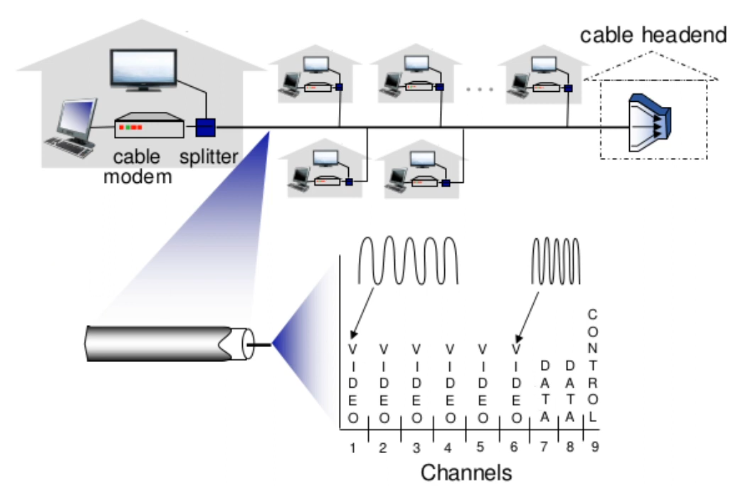
\includegraphics[width=0.6\textwidth]{img/cap-01/tv-a-cabo.png}
        \caption{Rede de acesso via TV a cabo (FDM).}
    \end{figure}

    \begin{figure}[H]
        \centering
        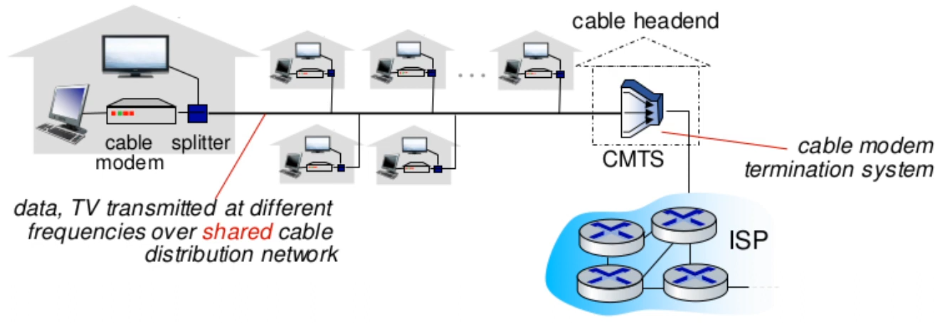
\includegraphics[width=0.6\textwidth]{img/cap-01/tv-a-cabo2.png}
        \caption{Arquitetura HFC híbrida coaxial-fibra.}
    \end{figure}

    \begin{itemize}
        \item Utiliza-se \textbf{HFC (Hybrid Fiber Coaxial)}, uma solução híbrida : \\
            $\hookrightarrow$ O \textbf{cabo coaxial} vai até o usuário. \\
            $\hookrightarrow$ A \textbf{interconexão} da rede é feita usando \textbf{fibra óptica}.
        \item \textbf{Assimétrica}: a capacidade de download e upload são diferentes.
        \item \textbf{Meio compartilhado}: o enlace é compartilhado entre vários usuários domésticos.
    \end{itemize}

    \paragraph{Rede baseada em DSL (\textit{Digital Subscriber Line})}
    \begin{itemize}
        \item Utiliza os \textbf{cabos telefônicos} como infraestrutura de enlace.
        \item A conexão \underline{não é compartilhada}.
        \item \textbf{Assimétrica} — download e upload possuem taxas diferentes.
    \end{itemize}

    \begin{figure}[H]
        \centering
        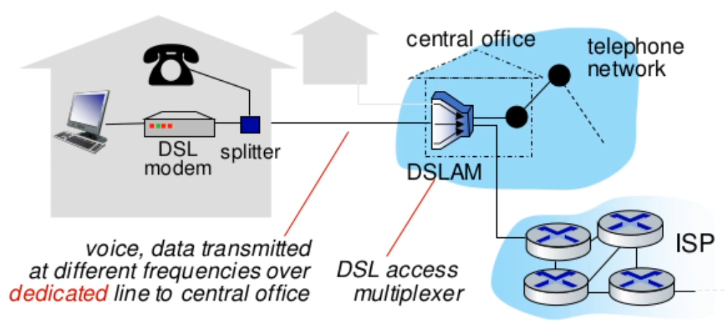
\includegraphics[width=0.6\textwidth]{img/cap-01/dsl.png}
        \caption{Rede DSL utilizando a infraestrutura telefônica.}
    \end{figure}

    {\textbf{Rede Doméstica}}

    \begin{figure}[H]
        \centering
        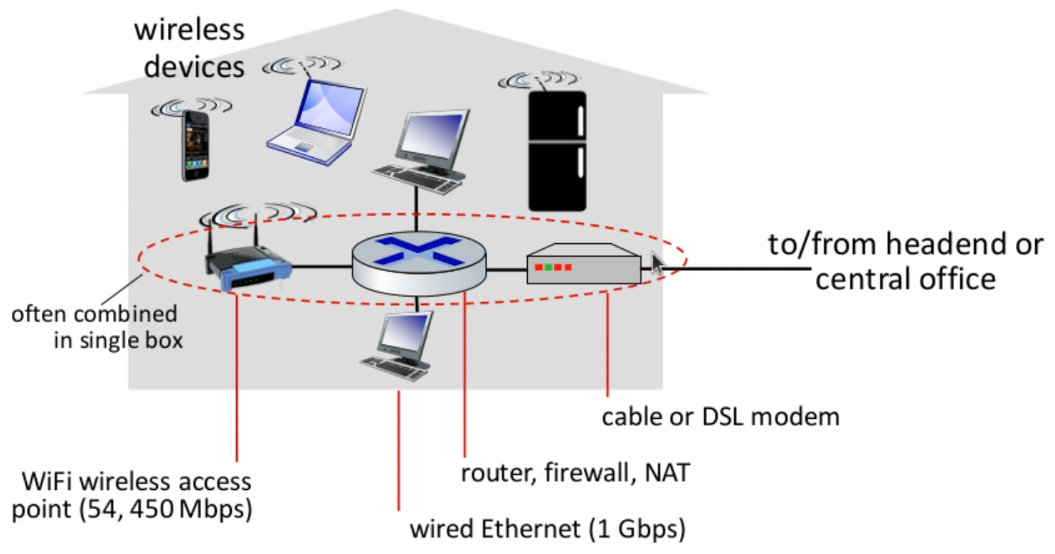
\includegraphics[width=0.6\textwidth]{img/cap-01/rede-domestica.png}
        \caption{Exemplo de rede doméstica.}
    \end{figure}

    \paragraph{Redes de Acesso Sem Fio (Wireless)}
    \begin{itemize}
        \item O \textbf{roteador de borda} é conectado a um \textbf{ponto de acesso}.
        \item \textbf{Locais}: alcance reduzido (domésticas, empresas) — \textbf{WiFi}.
        \item \textbf{Longas distâncias}: móveis (4G/5G), com pontos de acesso em \textbf{torres}, menor capacidade de transmissão.
    \end{itemize}

    \paragraph{Redes de Acesso Institucionais}
    \begin{itemize}
        \item Utilizadas em \textbf{universidades}, \textbf{empresas}, etc.
        \item Maior complexidade de interconexão — acesso sem fio conectado a switches e roteadores.
        \item Tecnologias utilizadas : \\
            $\hookrightarrow$ \textbf{Ethernet} \\
            $\hookrightarrow$ \textbf{WiFi}
    \end{itemize}

    \begin{figure}[H]
        \centering
        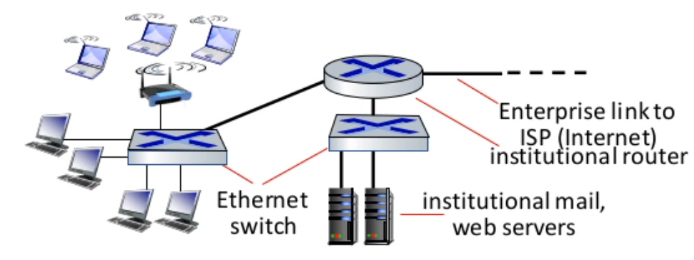
\includegraphics[width=0.6\textwidth]{img/cap-01/rede-institucional.png}
        \caption{Rede de acesso institucional.}
    \end{figure}

    \subsubsection*{Hosts (Sistemas Finais)}
    \begin{itemize}
        \item Quando o \textbf{host} tem conectividade, é possível enviar \textbf{pacotes de dados} até o destinatário.
        \item \textbf{Função de envio :} \\
            $\hookrightarrow$ Pega uma \textbf{mensagem} de uma aplicação.
            $\hookrightarrow$ Quebra essa mensagem em \textbf{pacotes menores} de tamanho $L$ bits.
            $\hookrightarrow$ Esses pacotes são transmitidos a uma taxa de transmissão $R$ (\textbf{bits/s}), correspondente à capacidade do enlace.
        \item \underline{Tempo de retardo (delay)} = tempo necessário para transmitir um pacote:  
        \[
        \text{delay} = \frac{L (\text{bits})}{R (\text{bits/s})}
        \]
    \end{itemize}

    \subsubsection*{Links (Enlaces)}
    \begin{itemize}
        \item Utilizados para a \textbf{interconexão de dispositivos}.
        \item Caracterizados por propriedades físicas.
        \item O \textbf{bit} é propagado entre transmissor e receptor.
        \item \textbf{Tipos de enlaces :} \\
            $\hookrightarrow$ \textbf{Guiados}: sinal se propaga em meio sólido (fibra óptica, cabos coaxiais, par trançado). \\
            \textbf{Não guiados}: sinal se propaga de forma livre (ondas eletromagnéticas). 
    \end{itemize}

    \paragraph{Cabos Par Trançado (Twisted Pair - TP)}
    
        $bullet$ Categorias mais comuns: \textbf{Cat 5}, \textbf{Cat 6}.
    
    \begin{figure}[H]
        \centering
        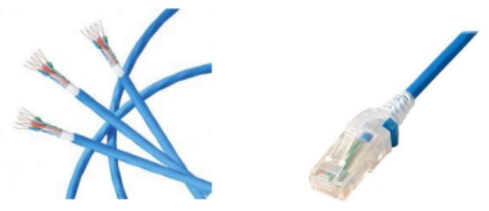
\includegraphics[width=0.6\textwidth]{img/cap-01/cabos-tp.png}
        \caption{Cabos Par Trançado (Twisted Pair).}
    \end{figure}

    \paragraph{Cabos Coaxiais}
    \begin{itemize}
        \item Dois condutores de cobre concêntricos.
        \item \textbf{Bidirecional}: transmite e recebe dados simultaneamente.
        \item Suporta \textbf{conexão de banda larga} — coexistência de múltiplas frequências no mesmo cabo.
    \end{itemize}

    \begin{figure}[H]
        \centering
        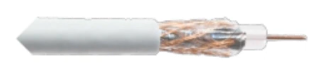
\includegraphics[width=0.6\textwidth]{img/cap-01/cabo-coaxial.png}
        \caption{Estrutura de um cabo coaxial.}
    \end{figure}

    \paragraph{Cabos de Fibra Óptica}
    \begin{itemize}
        \item Feitos de \textbf{vidro}.
        \item Transmissão em \textbf{alta velocidade} e \textbf{longa distância}.
        \item \textbf{Taxa de erro muito baixa}, dispensando regeneração do sinal.
        \item Imunes a \textbf{ruídos eletromagnéticos}.
    \end{itemize}

    \begin{figure}[H]
        \centering
        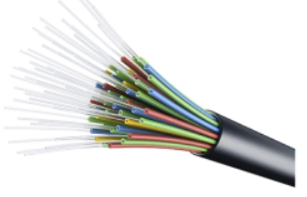
\includegraphics[width=0.6\textwidth]{img/cap-01/fibra-optica.png}
        \caption{Cabo de fibra óptica.}
    \end{figure}

    \paragraph{Transmissão via Rádio}
    \begin{itemize}
        \item Sinal transmitido no \textbf{espectro eletromagnético}.
        \item Comunicação \textbf{sem fio} e geralmente em modo \textbf{broadcast} (difusão).
        \item Operação \textbf{half-duplex}: alterna entre receber e enviar informações.
        \item \textbf{Problemas comuns de transmissão :} \\
            $\hookrightarrow$ Reflexão \\
            $\hookrightarrow$ Obstrução por objetos \\
            $\hookrightarrow$ Interferência 
        \item \textbf{Tipos de transmissão via rádio :} \\
            $\hookrightarrow$ Micro-ondas terrestres \\
            $\hookrightarrow$ \textbf{Wireless LAN} (WiFi) \\
            $\hookrightarrow$ \textbf{Sem fio de longo alcance} (4G/5G) \\
            $\hookrightarrow$ \textbf{Satélite} — possui \underline{retardo de transmissão elevado}.
    \end{itemize}

    \subsection{Núcleo da Rede}

    \begin{itemize}
        \item Parte \textbf{central da rede}, responsável por interconectar as redes de acesso.
        \item É composta por uma \textbf{malha de roteadores interconectados} que realizam o \textbf{encaminhamento de pacotes de dados} gerados pelos sistemas finais.
    \end{itemize}

    \subsubsection*{Comutação de Pacotes (\textit{Packet Switching})}
    \begin{itemize}
        \item O \textbf{sistema final} divide a \textbf{mensagem da aplicação} em \textbf{pacotes}.
        \item Esses pacotes são encaminhados \underline{roteador a roteador}, seguindo um caminho até o destino.
        \item Cada pacote é transmitido utilizando \textbf{toda a capacidade do enlace} entre os roteadores.
    \end{itemize}

    \begin{figure}[H]
        \centering
        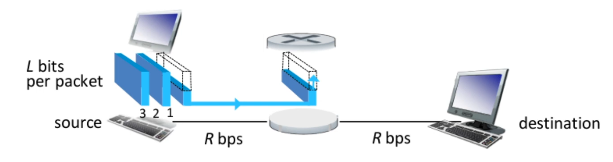
\includegraphics[width=0.55\textwidth]{img/cap-01/retardo.png}
        \caption{Encaminhamento de pacotes e retardo na transmissão.}
    \end{figure}

    \begin{itemize}
        \item Cada pacote passa por uma série de roteadores desde a origem até o destino.
        \item Em cada roteador é necessário que o pacote seja \textbf{recebido completamente} antes de ser retransmitido.
        \item \underline{Delay fim-a-fim}: $2L/R$ (assumindo delay de propagação nulo).
        \item \textbf{Exemplo:} $L = 10$ Kbits, $R = 100$ Mbps $\Rightarrow$ cada salto de transmissão leva $0.1$ ms.
    \end{itemize}

    \paragraph{Atrasos e Perdas (\textit{Queueing Delay, Loss})}
    \begin{itemize}
        \item Quando a \textbf{taxa de chegada} de pacotes em um roteador excede a \textbf{taxa de saída}, ocorre o \underline{enfileiramento}.
        \item Pacotes são \textbf{enfileirados} aguardando o enlace ficar livre — adicionando retardo ao processo de transmissão fim a fim.
        \item Caso a fila de saída esteja cheia, os pacotes são \textbf{descartados (perdidos)}.
    \end{itemize}

    \begin{figure}[H]
        \centering
        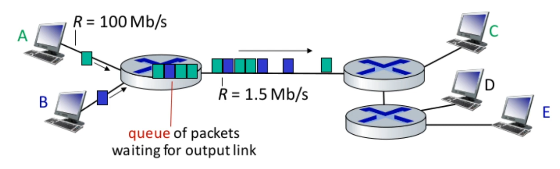
\includegraphics[width=0.55\textwidth]{img/cap-01/fila-e-perda.png}
        \caption{Fila de pacotes e perdas em roteadores.}
    \end{figure}

    \subsubsection*{Funções Principais do Núcleo da Rede}
    \begin{itemize}
        \item \textbf{Encaminhamento (Forwarding):} ação \underline{local} — move pacotes do enlace de entrada para o enlace de saída apropriado.
        \item \textbf{Roteamento (Routing):} ação \underline{global} — define os caminhos de origem a destino dentro da rede, utilizando \textbf{algoritmos de roteamento}.
    \end{itemize}

    \begin{figure}[H]
        \centering
        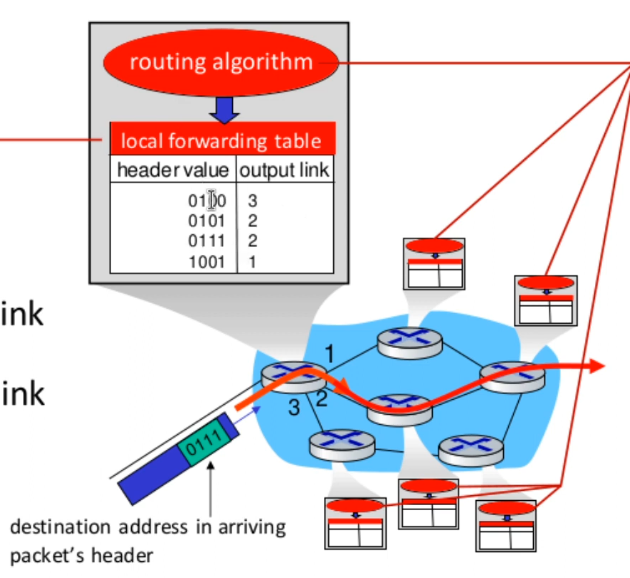
\includegraphics[width=0.55\textwidth]{img/cap-01/encaminhamento-roteamento.png}
        \caption{Diferença entre encaminhamento e roteamento.}
    \end{figure}

    \subsubsection*{Alternativa: Comutação por Circuito}
    \begin{itemize}
        \item Na comutação por circuito, existe uma \textbf{etapa inicial de conexão} onde : \\        
            $\hookrightarrow$ É definida a rota completa do início ao fim. \\
            $\hookrightarrow$ São \textbf{alocados recursos} nos roteadores ao longo do caminho. \\
            $\hookrightarrow$ Cada roteador envolvido armazena informação sobre essa rota. 
        \item Os pacotes transportam a informação sobre o \textbf{circuito virtual} ao qual pertencem.
    \end{itemize}

    \begin{figure}[H]
        \centering
        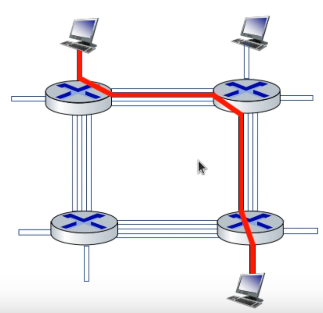
\includegraphics[width=0.55\textwidth]{img/cap-01/comutacao-circuitos.png}
        \caption{Comutação por circuito.}
    \end{figure}

    \paragraph{Técnicas de Multiplexação}
    \begin{itemize}
        \item \textbf{Frequency Division Multiplexing (FDM) :} \\
            $\hookrightarrow$ Divide a capacidade do enlace em \textbf{faixas de frequência}. \\
            $\hookrightarrow$ Cada faixa é dedicada a um usuário, transmitindo até a taxa máxima da sua banda.
        
        \begin{figure}[H]
            \centering
            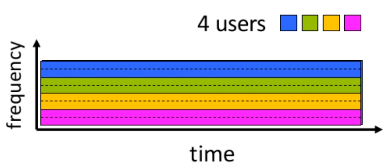
\includegraphics[width=0.55\textwidth]{img/cap-01/multiplexicacao-por-frequencia.png}
            \caption{Multiplexação por frequência (FDM).}
        \end{figure}

        \item \textbf{Time Division Multiplexing (TDM) :} \\
            $\hookrightarrow$ Divide o tempo de transmissão em \textbf{intervalos (slots)}. \\
            $\hookrightarrow$ Cada usuário transmite à taxa total do enlace durante o seu slot de tempo.
        
        \begin{figure}[H]
            \centering
            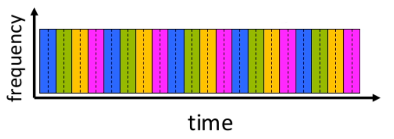
\includegraphics[width=0.55\textwidth]{img/cap-01/multiplexicacao-por-tempo.png}
            \caption{Multiplexação por tempo (TDM).}
        \end{figure}
    \end{itemize}

    \paragraph{Comparação: Comutação de Pacotes vs. Comutação de Circuitos}
    \begin{itemize}
        \item Ambas possuem a mesma \textbf{taxa de transmissão nominal}.
        \item A \textbf{comutação de pacotes} permite que mais usuários utilizem a rede simultaneamente.
        \item É mais eficiente para \textbf{“bursty data”} (rajadas de dados) : \\    
            $\hookrightarrow$ Melhor \textbf{compartilhamento de recursos}.
            $\hookrightarrow$ Operação mais \textbf{simples}, sem necessidade de estabelecimento de chamada.
        
        \item \textbf{Problema :} Ausência de controle de congestionamento. \\
            $\hookrightarrow$ Pode causar aumento de retardo e perda de pacotes devido ao transbordo das filas. \\
            $\hookrightarrow$ Protocolos específicos são utilizados para controle de congestionamento.
        
        \item Aplicações como \textbf{vídeo/áudio streaming} ainda utilizam comutação de circuitos.
    
    \end{itemize}

    \subsubsection*{Estrutura da Internet}
    \begin{itemize}
        \item Os \textbf{hosts} se conectam à Internet por meio de \textbf{provedores de acesso (ISPs)} : \\
            $\hookrightarrow$ Domésticos, empresariais ou institucionais.
        \item Esses provedores precisam se \textbf{interconectar} para permitir comunicação entre seus clientes.
        \item Isso resultou em uma rede de \textbf{alta complexidade}, moldada por \textbf{decisões econômicas e políticas}.
    \end{itemize}

    \begin{figure}[H]
        \centering
        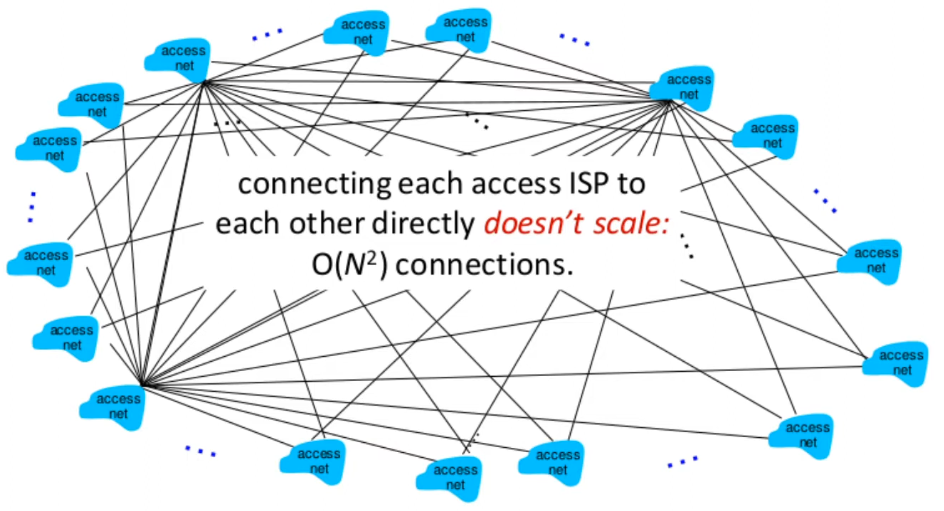
\includegraphics[width=0.55\textwidth]{img/cap-01/infraestrutura1.png}
        \caption{Evolução da infraestrutura da Internet.}
    \end{figure}

    \paragraph{Hierarquização da Conexão}
    \begin{itemize}
        \item Solução: criar um \textbf{provedor de acesso global}.
        \item Provedores locais se conectam a ele, estabelecendo uma relação \textbf{econômica} (pagamento pelo uso do serviço de trânsito).
    \end{itemize}

    \begin{figure}[H]
        \centering
        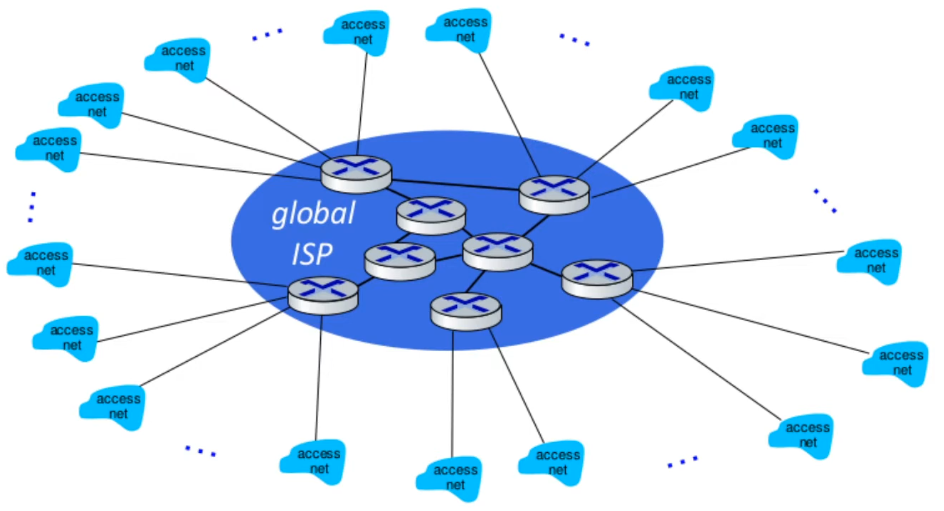
\includegraphics[width=0.55\textwidth]{img/cap-01/infraestrutura2.png}
        \caption{Conexão hierárquica entre provedores locais e globais.}
    \end{figure}

    \begin{itemize}
        \item Com o tempo, surgiu \textbf{concorrência} tanto por questões econômicas quanto geográficas.
    \end{itemize}

    \begin{figure}[H]
        \centering
        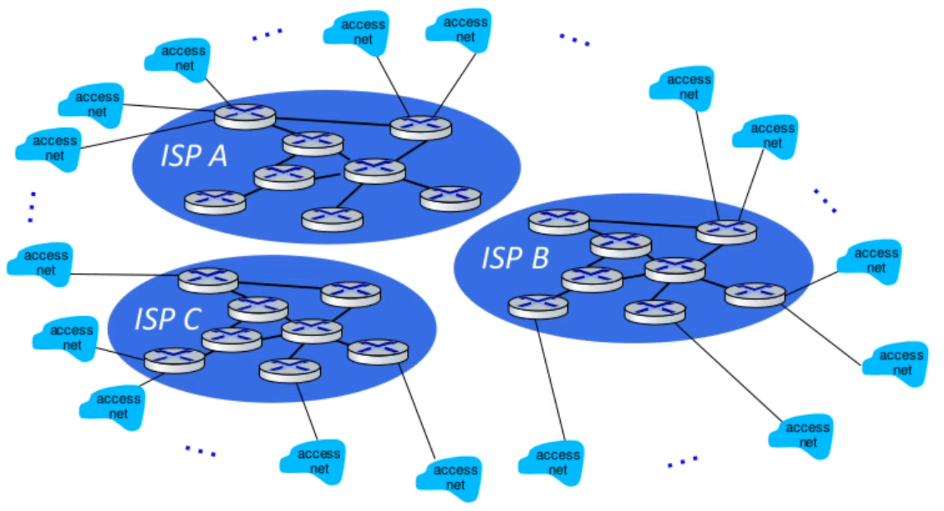
\includegraphics[width=0.55\textwidth]{img/cap-01/infraestrutura3.png}
        \caption{Concorrência e distribuição geográfica de provedores.}
    \end{figure}

    \paragraph{Peering e Pontos de Troca de Tráfego}
    \begin{itemize}
        \item A conexão entre provedores locais ocorre por meio de : \\
            $\hookrightarrow$ \textbf{Peering físico (peering link)} \\
            $\hookrightarrow$ \textbf{Pontos de Troca de Tráfego (IXP)}
    \end{itemize}

    \begin{figure}[H]
        \centering
        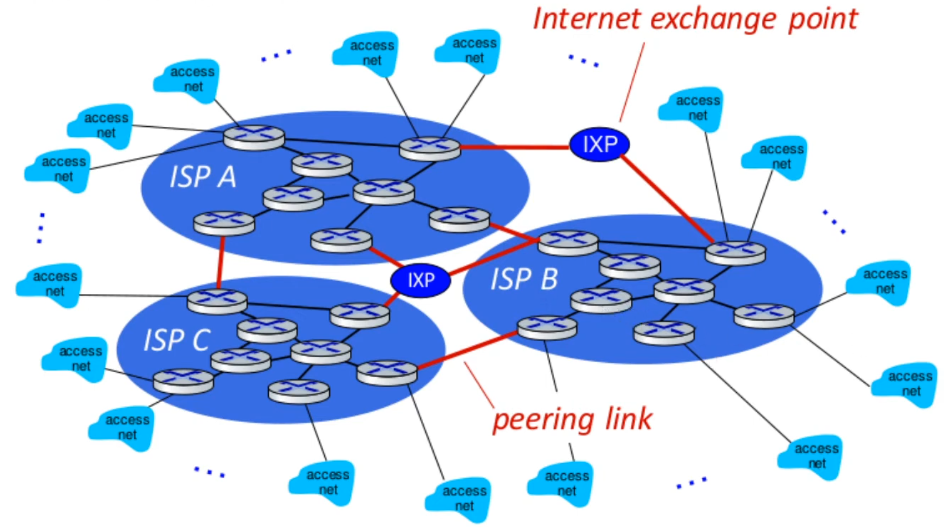
\includegraphics[width=0.55\textwidth]{img/cap-01/infraestrutura4.png}
        \caption{Conexão entre provedores locais e IXP.}
    \end{figure}

    \paragraph{Provedores Regionais e Globais}
    \begin{itemize}
        \item Devido à distância geográfica entre provedores globais e locais, surgiram \textbf{provedores regionais}.
        \item Grandes provedores de conteúdo (\textbf{Google, Microsoft, etc.}) se conectam diretamente aos provedores globais.
    \end{itemize}

    \begin{figure}[H]
        \centering
        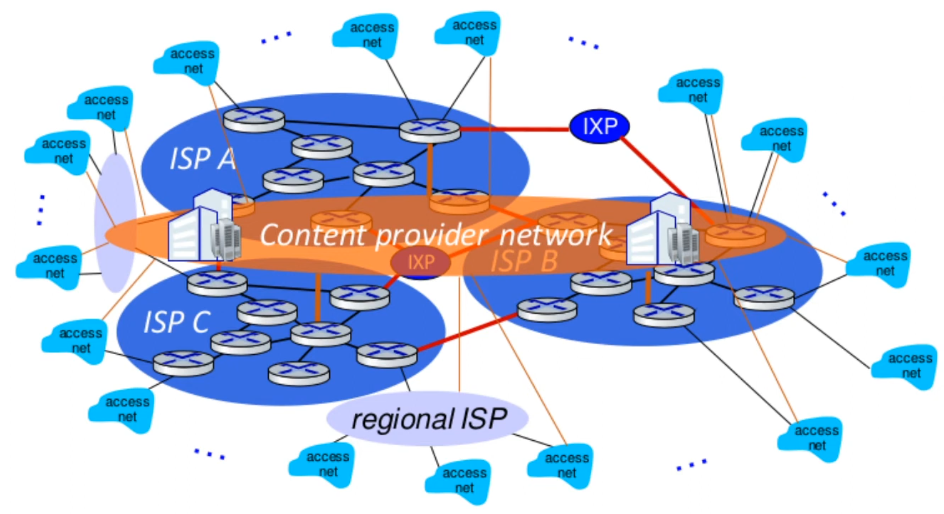
\includegraphics[width=0.55\textwidth]{img/cap-01/infraestrutura5.png}
        \caption{Conexão de provedores de conteúdo com provedores globais.}
    \end{figure}

    \paragraph{Hierarquia da Internet}
    \begin{figure}[H]
        \centering
        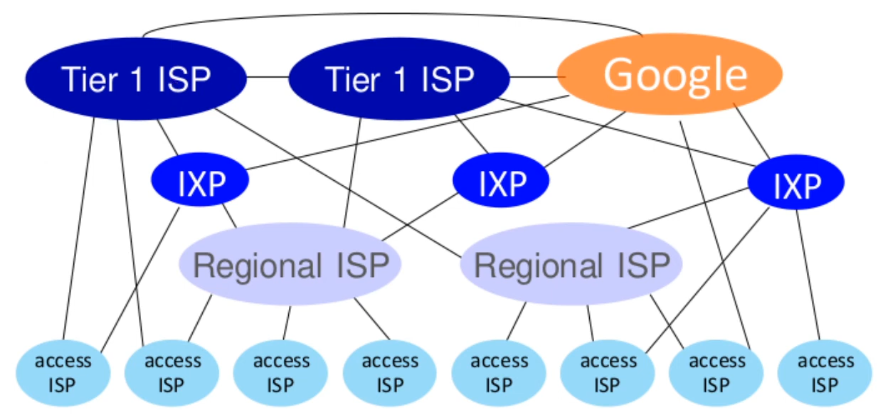
\includegraphics[width=0.55\textwidth]{img/cap-01/hierarquia.png}
        \caption{Hierarquia dos provedores de acesso à Internet.}
    \end{figure}

   \subsection{Performance}

    \begin{itemize}
        \item \textbf{Como ocorre a perda e o retardo de pacotes ?} \\
            $\hookrightarrow$ Pacotes enfileirados esperam a sua vez de serem transmitidos. \\
            $\hookrightarrow$ \textbf{Retardo de enfileiramento}: \underline{tempo que um pacote aguarda na fila} para ser transmitido. \\
            $\hookrightarrow$ \textbf{Retardo de transmissão}: \underline{tempo que leva para transmitir os bits} no enlace. \\
            $\hookrightarrow$ Se a \textbf{taxa de chegada} no enlace (temporariamente) excede a capacidade de saída, ocorre a \textbf{perda de pacotes}. 
      

        \begin{center}
            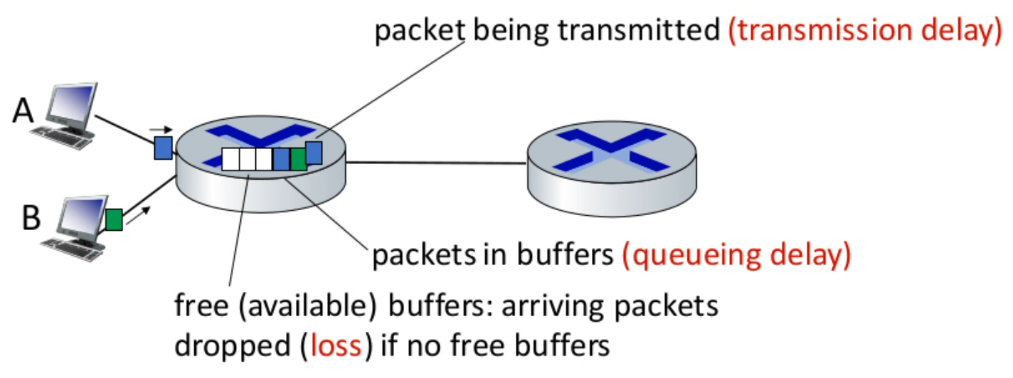
\includegraphics[width=0.6\textwidth]{img/cap-01/delay1.png}
        \end{center}

        \item \textbf{Retardo do Pacote: 4 Causas}
            $\hookrightarrow$ O retardo ocorre a cada nó (ou salto) na rede : 
            \[
            d_{nodal} = d_{proc} + d_{queue} + d_{trans} + d_{prop}
            \]
        

        \begin{center}
            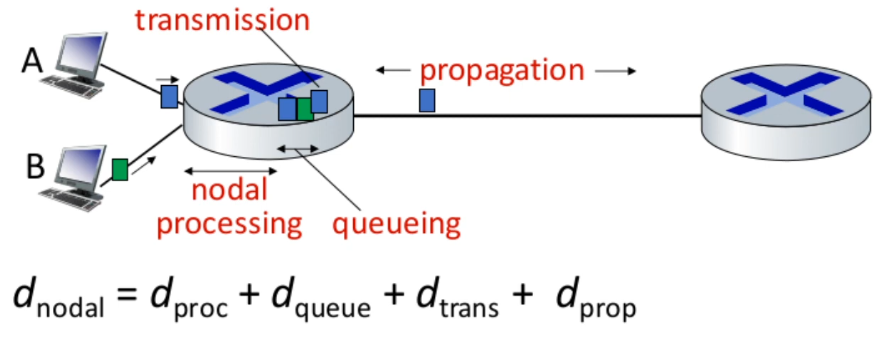
\includegraphics[width=0.7\textwidth]{img/cap-01/delay2.png}
        \end{center}

        \item \textbf{Componentes do Retardo :}
        
            $\hookrightarrow$ \textbf{$d_{proc}$ — Retardo de Processamento do Nó :}
            \begin{itemize}
                \item Tempo gasto pelo roteador para processar o pacote que acabou de chegar.
                \item Envolve tarefas como:
                \begin{itemize}
                    \item Conferir a integridade do pacote.
                    \item Verificar o endereço de saída do pacote.
                \end{itemize}
                \item Geralmente menor que 1 ms.
            \end{itemize}

            $\hookrightarrow$ \textbf{$d_{queue}$ — Retardo de Enfileiramento :}
            \begin{itemize}
                \item Tempo que o pacote aguarda na fila antes da transmissão.
                \item Depende do \textbf{nível de congestionamento} no roteador.
            \end{itemize}

            $\hookrightarrow$ \textbf{$d_{trans}$ — Retardo de Transmissão :}
            \begin{itemize}
                \item Tempo necessário para transmitir um pacote no enlace.
                \item Dados:
                \[
                L = \text{tamanho do pacote (bits)}, \quad R = \text{taxa de transmissão (bps)}
                \]
                \item Fórmula:
                \[
                d_{trans} = \frac{L}{R}
                \]
            \end{itemize}

            $\hookrightarrow$ \textbf{$d_{prop}$ — Retardo de Propagação :}
            \begin{itemize}
                \item Tempo necessário para que os bits do pacote \underline{propaguem até o destino}.
                \[
                d = \text{comprimento do enlace}, \quad s = \text{velocidade de propagação} \approx 2 \times 10^8 \text{ m/s}
                \]
                \item Fórmula:
                \[
                d_{prop} = \frac{d}{s}
                \]
            \end{itemize}
        
        \item \textbf{Exemplo: Caravanas de Carros}
        
            $\hookrightarrow$ Analogia :
            \begin{itemize}
                \item \textbf{1 Carro} $\rightarrow$ 1 \textbf{bit}.
                \item \textbf{Caravana} $\rightarrow$ \textbf{pacote}.
                \item \textbf{Pedágio} $\rightarrow$ \textbf{roteador}.
                \item \textbf{Estrada} $\rightarrow$ \textbf{enlace}.
            \end{itemize}
            
            $\hookrightarrow$ O pedágio leva 12 s para atender cada carro (tempo de transmissão). \\
            $\hookrightarrow$ A estrada tem pedágios a cada 100 km. \\
            $\hookrightarrow$ Um carro se propaga a 100 km/h. \\
            $\hookrightarrow$ \textbf{Pergunta 1:} Quanto tempo levaria para a caravana de 10 carros chegar ao 2º pedágio ? 
            
            \begin{itemize}
                \item Tempo de transmissão: $12 \times 10 = 120$ s.
                \item Tempo de propagação: $100$ km / $100$ km/h = 1 h.
                \item Tempo total: \textbf{62 minutos}.
            \end{itemize}
            $\hookrightarrow$ \textbf{Pergunta 2:} Se os carros se propagam a 1000 km/h e o pedágio leva 1 min por carro?
            \begin{itemize}
                \item Tempo de propagação: 6 min.
                \item O primeiro carro chega ao segundo pedágio após 7 min, antes de todos terminarem no primeiro pedágio.
            \end{itemize}
        \end{itemize}

        \begin{center}
            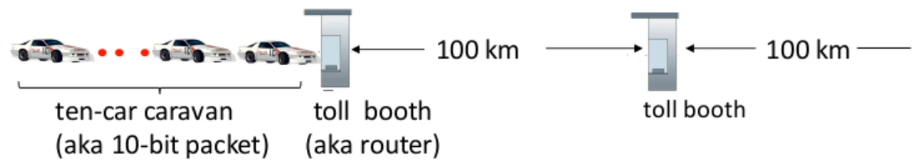
\includegraphics[width=0.7\textwidth]{img/cap-01/carro-pedagio.png}
        \end{center}

        $\hookrightarrow$ \textbf{Revisão: Retardo de Enfileiramento}
        
        $R = \text{Capacidade de transmissão (bps)}$ \\ 
        $L = \text{Tamanho do pacote (bits)}$ \\
        $a = \text{Taxa de chegada (pacotes/s)}$
        
        \begin{itemize}
            \item $La/R \approx 0$: retardo pequeno.
            \item $La/R \rightarrow 1$: retardo grande.
            \item $La/R > 1$: \underline{taxa de chegada maior que a capacidade de transmissão}, retardo tende ao infinito.
        \end{itemize}

        \begin{center}
            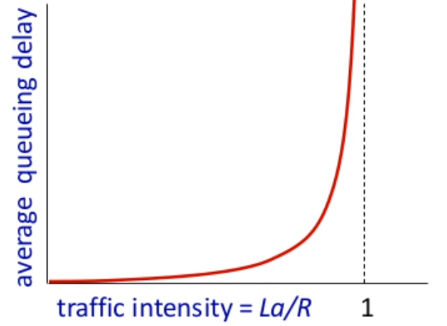
\includegraphics[width=0.6\textwidth]{img/cap-01/retardo-de-enfileiramento.png}
        \end{center}

        $\hookrightarrow$ \textbf{Exemplo Real — \texttt{traceroute}}
        \begin{itemize}
            \item Programa que permite \underline{avaliar cada roteador} ao longo da rota seguida pelos pacotes.
            \item Mostra o \textbf{tempo de ida e volta (RTT)} de cada salto.
        \end{itemize}

        \begin{center}
            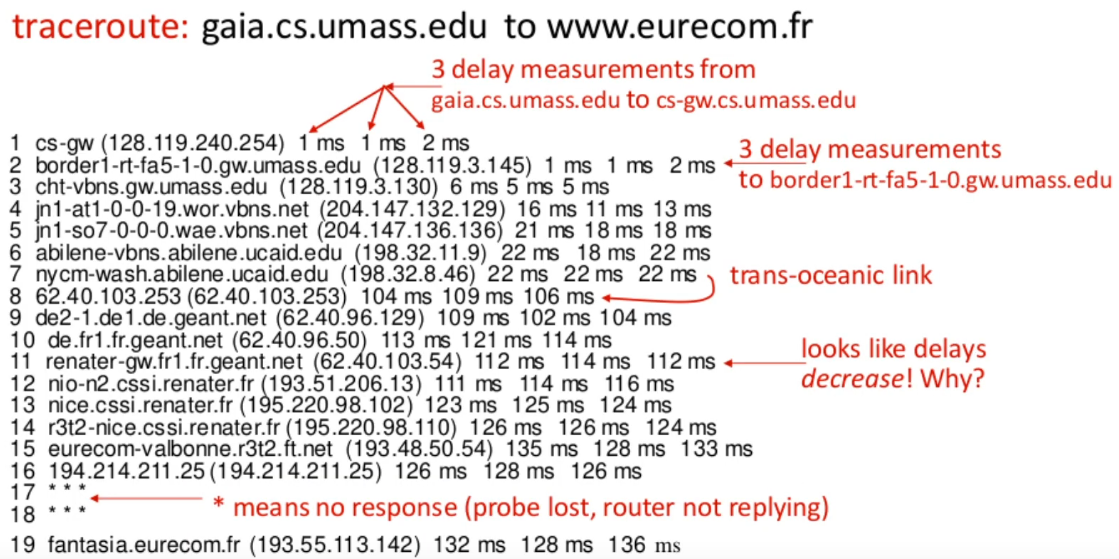
\includegraphics[width=0.7\textwidth]{img/cap-01/traceroute-exemplo.png}
        \end{center}

        $\hookrightarrow$ \textbf{Perda de Pacotes}
        \begin{itemize}
            \item A fila (\textbf{buffer}) precede um enlace de saída.
            \item Quando a fila está cheia, o pacote é \underline{descartado}.
            \item Pacotes perdidos precisam ser \textbf{retransmitidos}.
        \end{itemize}

        \begin{center}
            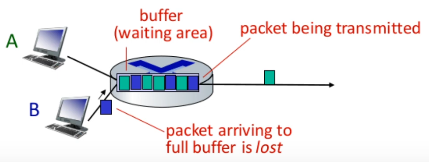
\includegraphics[width=0.6\textwidth]{img/cap-01/perda-de-pacotes.png}
        \end{center}

        $\hookrightarrow$ \textbf{Vazão (Throughput)}
        \begin{itemize}
            \item \textbf{Throughput}: \underline{taxa de transmissão efetiva} percebida por uma conexão.
            \item Tipos:
            \begin{itemize}
                \item \textbf{Instantânea}: medida em um determinado instante.
                \item \textbf{Média}: média ao longo de um período.
            \end{itemize}
            \item A vazão é sempre limitada pelo \textbf{link gargalo}.
        \end{itemize}

        \begin{center}
            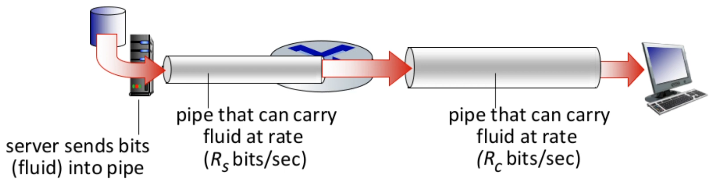
\includegraphics[width=0.6\textwidth]{img/cap-01/vazao.png}
        \end{center}

        \begin{center}
            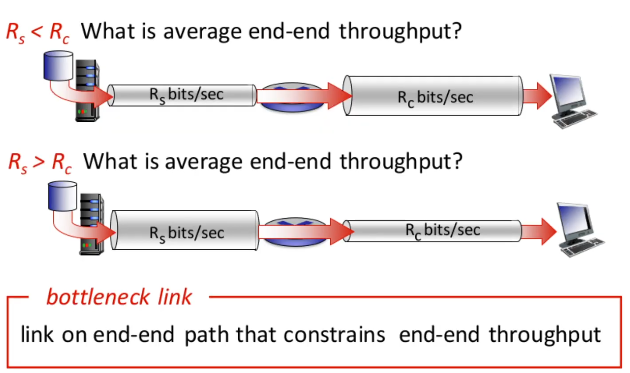
\includegraphics[width=0.6\textwidth]{img/cap-01/exemplo-vazao.png}
        \end{center}

        \begin{center}
            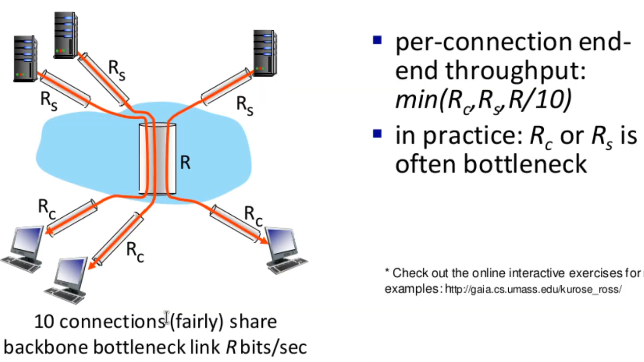
\includegraphics[width=0.6\textwidth]{img/cap-01/exemplo-vazao2.png}
        \end{center}

    \subsection{Camadas de Protocolos e Modelos de Serviços}

    \begin{itemize}
        \item \textbf{Questão inicial:} Existia alguma maneira de organizar a estrutura da Internet?

        \item \textbf{Exemplo: Organização para Viajar de Avião} \\
            $\hookrightarrow$ Uma viagem de avião envolve uma série de etapas e serviços distintos. \\
            $\hookrightarrow$ Cada etapa pode ser vista como uma \textbf{camada}, responsável por uma parte específica do processo.
        

        \begin{figure}[H]
            \centering
            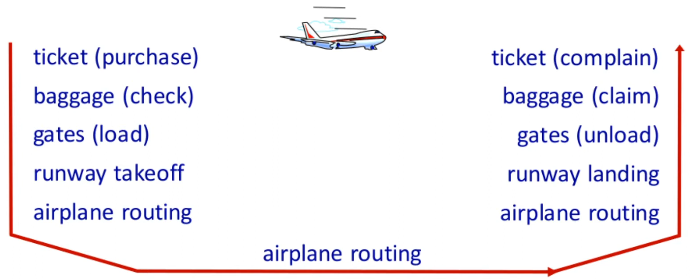
\includegraphics[width=0.6\textwidth]{img/cap-01/exemplo-aviao.png}
            \caption{Organização em etapas de uma viagem de avião.}
        \end{figure}

        \item \textbf{Camadas :} \\ 
            $\hookrightarrow$ Cada camada implementa um \textbf{serviço} específico. \\
            $\hookrightarrow$ Cada camada tem uma \textbf{contrapartida} tanto na origem quanto no destino.
        
        \begin{figure}[H]
            \centering
            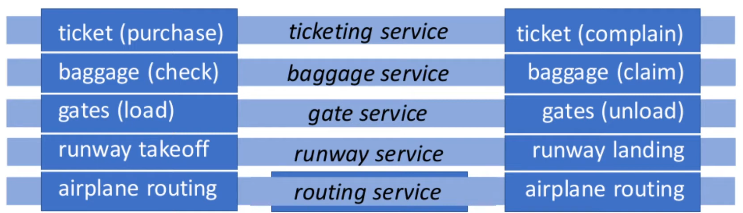
\includegraphics[width=0.6\textwidth]{img/cap-01/exemplo-aviao2.png}
            \caption{Camadas de serviço e suas contrapartidas.}
        \end{figure}

        \item \textbf{Por que usar camadas ?} \\
            $\hookrightarrow$ A ideia surge naturalmente em sistemas complexos. \\
            $\hookrightarrow$ \textbf{Abstrai} partes do sistema em diferentes camadas. \\
            $\hookrightarrow$ Cada camada deve ser \textbf{bem definida} e possuir uma \textbf{interface clara}. \\
            $\hookrightarrow$ Facilita a \textbf{modularização}, \textbf{manutenção} e \textbf{atualização} do sistema. \\
            $\hookrightarrow$ \underline{Problema:} pode haver \textbf{redundância de ações} entre camadas.

        \item \textbf{Pilha de Protocolos da Internet (TCP/IP)}
        
            $\hookrightarrow$ \textbf{Aplicação :} Suporta as aplicações que estão executando nos sistemas finais.
            \begin{itemize}
                \item Exemplos: \texttt{HTTP}, \texttt{SMTP}, \texttt{IMAP}.
            \end{itemize}
            
            $\hookrightarrow$ \textbf{Transporte :} Responsável pela \textbf{transferência de pacotes entre processos} que estão executando nos sistemas finais.
            \begin{itemize}
                \item Exemplos: \texttt{UDP}, \texttt{TCP}.
            \end{itemize}

            $\hookrightarrow$ \textbf{Rede :} Faz o \textbf{roteamento dos pacotes} da origem até o destino.
            \begin{itemize}
                \item Exemplos: \texttt{IP}, \texttt{Protocolos de roteamento}.
            \end{itemize}

            $\hookrightarrow$ \textbf{Enlace :} Garante a \textbf{transferência de dados entre dispositivos diretamente conectados}.
            \begin{itemize}
                \item Exemplos: \texttt{Ethernet}, \texttt{802.11 (WiFi)}, \texttt{PPP}.
            \end{itemize}

            $\hookrightarrow$ \textbf{Física :} Responsável pela \textbf{transmissão dos bits} através do meio físico.
        

        \begin{center}
            \begin{tikzpicture}
                \node[draw, minimum width=4cm, minimum height=1cm, fill=blue!10] (app) {\textbf{Aplicação}};
                \node[draw, below=0cm of app, minimum width=4cm, minimum height=1cm, fill=green!10] (transp) {\textbf{Transporte}};
                \node[draw, below=0cm of transp, minimum width=4cm, minimum height=1cm, fill=yellow!10] (rede) {\textbf{Rede}};
                \node[draw, below=0cm of rede, minimum width=4cm, minimum height=1cm, fill=orange!10] (enlace) {\textbf{Enlace}};
                \node[draw, below=0cm of enlace, minimum width=4cm, minimum height=1cm, fill=red!10] (fisica) {\textbf{Física}};
            \end{tikzpicture}
        \end{center}

        \item \textbf{Encapsulamento :} \\
            $\hookrightarrow$ Cada camada adiciona seu próprio cabeçalho à unidade de dados recebida da camada superior. \\
            $\hookrightarrow$ O processo é \textbf{reverso} no destino: cada camada remove seu cabeçalho correspondente. \\
            $\hookrightarrow$ Esse mecanismo garante que cada camada só interaja com sua correspondente no outro sistema.
        
        \begin{figure}[H]
            \centering
            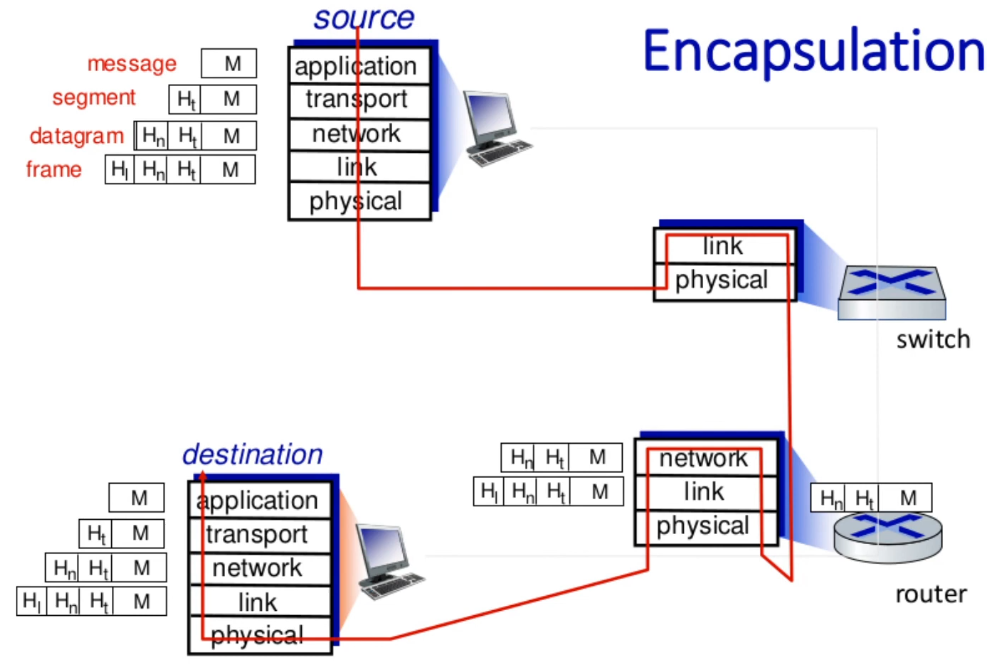
\includegraphics[width=0.65\textwidth]{img/cap-01/encapsulamento.png}
            \caption{Processo de encapsulamento nas camadas de protocolos.}
        \end{figure}
    \end{itemize}

\section{Lógica Proposicional}

\section{Teoria de Provas}

\section{Tableaux Proposicional}

\section{Lógica de Primeira Ordem}


\end{document}
